\chapter{Avaliação}
\label{c_avaliacao}
Este capítulo apresenta o contexto e os procedimentos metodológicos adotados nesta pesquisa. Ela tem abordagem qualitativa exploratória, e buscou gerar dados descritivos e explanatórios em vez de demonstrar relações estatísticas de causa e efeito.
O objetivo foi observar e descrever as interações das crianças com a RoPE AR durante a programação e depuração de algoritmos, em um ambiente educacional infantil, e captar as percepções de professores a respeito da proposta. Para isso, a \autoref{sec:contexto} descreve o contexto de realização da pesquisa e a \autoref{sec:participantes} descreve os participantes. Por fim, a \autoref{sec:protocolo} apresenta os experimentos realizados, detalhando a estratégia de coleta de dados e o método de análise destes dados.

\section{Contexto}
\label{sec:contexto}
\subsection{Município}\\
A coleta de dados ocorreu em um \ac{CDI} no município de Gaspar, no estado de Santa Catarina. Dados do IBGE (Instituto Brasileiro de Geografia e Estatística) permitem comparar o município em relação ao demais municípios do Brasil\footnote{\url{https://cidades.ibge.gov.br/brasil/sc/gaspar/panorama}}. Em aspectos populacionais, a cidade está entre as 10\% mais populosas do Brasil (70 mil habitantes). É um local com alta disponibilidade de emprego, estando entre as 5\% cidades brasileiras com maior ocupação (41,8\% da população). 

Quanto à saúde, a cidade tem uma taxa de 9,05 mortes a cada 1000 nascidos vivos, o que a coloca na metade inferior do ranking de municípios do Brasil. Por outro lado, está entre os 10\% de cidades brasileiras com maior cobertura de esgotamento sanitário (87,3\%).

Em aspectos educacionais, a taxa de escolarização entre 6 e 14 anos é 93,7\%, o que é próximo da média brasileira. Já o desempenho no \ac{IDEB} para anos iniciais é maior que 74\% dos municípios brasileiros, tendo nota 6,3. Essa nota diminui nos anos finais (4,7), tendência que também é acompanhada pelos demais municípios. 

Em resumo, em relação aos demais municípios, percebe-se que é Gaspar é uma cidade populosa, com condições sanitárias adequadas, escolarização média e desenvolvimento educacional de médio a alto. Certamente esses dados não permitem uma visão completa ou profunda do contexto municipal, mas permitem posicioná-lo em aspectos de população, saúde e educação em relação ao Brasil. A próxima seção aprofunda a descrição do CDI onde se deu a pesquisa.

\subsection{Centro de Desenvolvimento Infantil}
\label{sec:cdi}
A pesquisa ocorreu em um \ac{CDI} de um bairro urbano, distante aproximadamente cinco quilômetros do centro da cidade. O local foi selecionado por conveniência, facilitado pelo contato com uma professora que leciona no local, o que possibilitou pesquisas em anos anteriores. A pesquisa atual, entretanto, não ocorreu nas turmas desta professora. Além disso, nenhum dos participantes conhecia o brinquedo RoPE. Outro critério para a seleção do centro foi a presença de internet, dado que o projetor e a CtPuzzle Platform são acessíveis por conexão sem fio local.

O \ac{PPP} do \ac{CDI} apresenta dados históricos e da estrutura física do local. O mesmo foi fundado em 1990, sendo uma parceria entre a prefeitura municipal e a associação de moradores do bairro. Atualmente possui 38 colaboradores, que promovem o atendimento de 246 crianças. A idade atendida vai de zero e cinco anos e onze meses, e há 12 turmas organizadas em três grupos etários: Infância I (0 a 2 anos), Infância II (2 a 4 anos) e Infância III (4 a 6 anos). Dentro de cada grupo etário as turmas também são divididas. Na Infância III, por exemplo, há as turmas de 4 a 5 e de 5 a 6 anos. O espaço tem 9 salas onde as professoras realizam suas atividades, uma biblioteca com aproximadamente 300 livros infantis, um parquinho, banheiros, sala de coordenação e sala do zelador. Além das salas existentes, está em curso a construção de novos espaços no local onde antes havia o parquinho, o qual foi deslocado para um espaço ao lado do CDI. 

O \ac{PPP} do \ac{CDI} apresenta um diagnóstico da comunidade, construído a partir de um questionário. O trabalho apresenta gráficos de pizza, que serão analisados visualmente pois não apresentam dados numéricos (\autoref{fig:contexto_ppp}). Aproximadamente 2/3 das crianças mora com pai e mãe, metade vai de carro ao \ac{CDI}, e quase a metade não tem computador em casa. A respeito dos pais, a maior parte auxilia os filhos nas atividades do \ac{CDI} mas não tem disponibilidade em horário comercial. A renda de aproximadamente a metade das famílias é de 1 a 2 salários-mínimos, e de outra metade vai de 2 a 4.

\begin{figure}[!htbp]
    \centering
    \begin{subfigure}{.3\linewidth}
        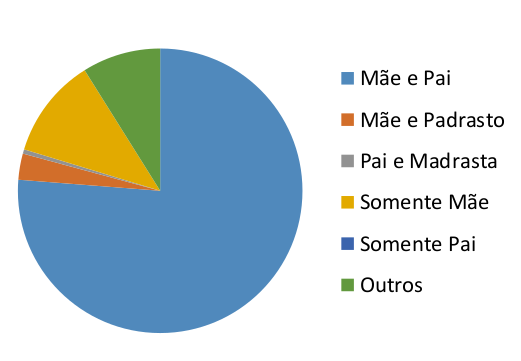
\includegraphics[width=.9\linewidth,fbox]{figs/cdi/mora_com.png}
        \caption{Com quem a criança mora.}
        \label{fig:mora_com}
    \end{subfigure}%
    \begin{subfigure}{.3\textwidth}
        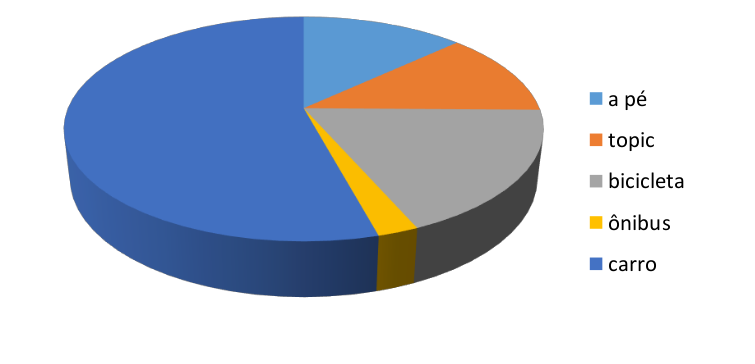
\includegraphics[width=.9\linewidth,fbox]{figs/cdi/meio_transporte.png}
        \caption{Meio de transporte.}
        \label{fig:transporte}
    \end{subfigure}%
   \begin{subfigure}{.3\textwidth}
        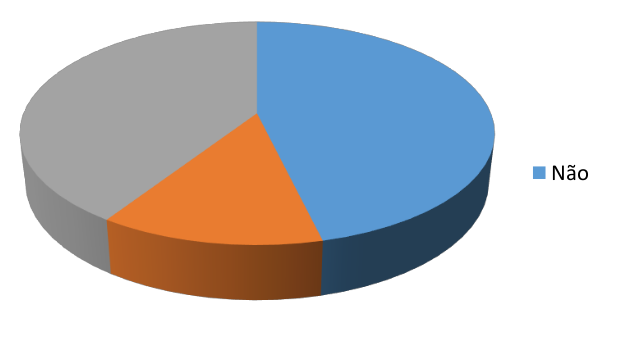
\includegraphics[width=.9\linewidth,fbox]{figs/cdi/tem_computador.png}
        \caption{Tem computador em casa?}
        \label{fig:tem_computador}
    \end{subfigure}
    \begin{subfigure}{.3\textwidth}
        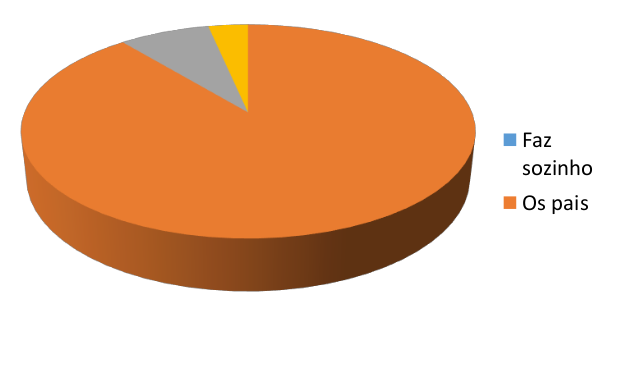
\includegraphics[width=.9\linewidth,fbox]{figs/cdi/pai_auxilia_crianca_atividades.png}
        \caption{Auxílio dos pais nas atividades do CDI}
        \label{fig:pai_auxilia_crianca_atividades}
    \end{subfigure}%
    \begin{subfigure}{.3\textwidth}
        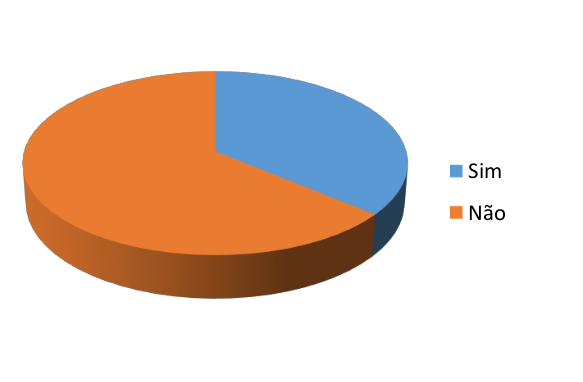
\includegraphics[width=.9\linewidth,fbox]{figs/cdi/disponibilidade_pais_horario_comercial.png}
        \caption{Disponibilidade dos pais em horário comercial.}
        \label{fig:disponibilidade_pais_horario_comercial}
    \end{subfigure}%
     \begin{subfigure}{.3\textwidth}
        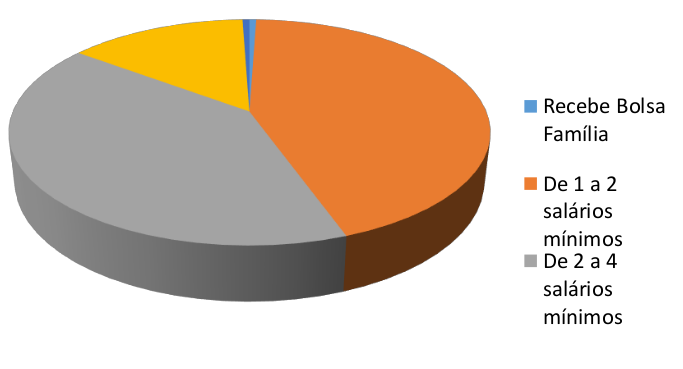
\includegraphics[width=.9\linewidth,fbox]{figs/cdi/renda.png}
        \caption{Renda mensal familiar.}
        \label{fig:renda}
    \end{subfigure}%
    \caption{Dados do Projeto Político Pedagógico do CDI.}
    \label{fig:contexto_ppp}
\end{figure}
Considerando os dados de ocupação da população, providos pelo IBGE, e os gráficos apresentados no \ac{PPP}, infere-se que as condições de vida na região não são precárias, porém a necessidade de trabalho impede o acompanhamento dos filhos em horário comercial. Em horário compatível, porém, os pais buscam auxiliar os filhos nas atividades escolares.

\subsection{Proposta Pedagógica para a Educação Infantil}
Mesmo com as suas particularidades locais, todos os CDIs de Gaspar buscam seguir uma mesma proposta pedagógica alinhada com a rede de ensino do municipal. O documento orientador é a Proposta Pedagógica da Rede Municipal para a Educação Infantil \cite{gaspar_proposta_2010}. Essa proposta foi publicada em 2010, após ser construída coletivamente pelos professores e professoras da Rede Municipal de Educação Infantil. O resultado é um documento que busca nortear o trabalho pedagógico “para e com” as crianças pequenas.

Este “norte” tem duas bases principais: os eixos de Linguagens, Interações e Brincadeiras, e a abordagem metodológica de projetos. Quanto aos eixos, o eixo de Linguagens tem como objetivo incrementar as aprendizagens infantis por meio de atividades que envolvam uso do corpo (linguagem motora); exploração dos sons (linguagem musical); exploração de cores, formas e texturas (linguagem plástica); fala e códigos (linguagem oral e escrita) e noções de espaço, quantidade e números (linguagem matemática). O eixo de Interações diz respeito ao planejamento e organização de situações de contato entre criança-criança, criança-adulto e criança-objeto. Por fim, o eixo das brincadeiras busca aumentar o repertório de interações lúdicas entre as crianças, orientando o educador a observar, coordenar ou integrar-se nas brincadeiras.

Já a Metodologia de Projetos, segundo a proposta, é uma abordagem que permite combinar as intenções pedagógicas do adulto e também estimular a curiosidade da criança. Esse estímulo se dá ao propor projetos em que há investigação de algum tema ou construção de algo com foco em assuntos do mundo infantil (ver \autoref{fig:tres_porquinhos}). Os temas dos projetos surgem em diálogos durante rodas de conversa, passeios ou brincadeiras. Partindo do interesse das crianças, os projetos seguem uma estrutura com hipóteses, perguntas de pesquisa, descrições e comparações. Não há prazo de início e fim, e também não há necessidade de trabalhar diariamente com projetos. Quando nenhum projeto está em curso, trabalha-se seguindo os eixos de Linguagens, Interações e Brincadeiras.

\begin{figure}[!h]
    \centering
    \begin{subfigure}{.45\linewidth}
        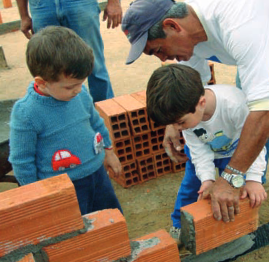
\includegraphics[width=.8\linewidth,fbox]{figs/tres_porquinhos.png}
        \caption{Projeto de construção de casa de tijolos (História dos Três Porquinhos).}
        \source{Proposta Pedagógica da Rede Municipal de Educação Infantil de Gaspar (2010). }
        \label{fig:tres_porquinhos}
    \end{subfigure}%
    \hspace{.05\textwidth}%
    \begin{subfigure}{.45\textwidth}
        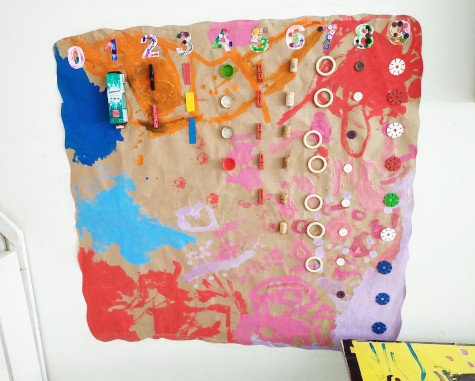
\includegraphics[width=.8\linewidth,fbox]{figs/projeto_numeros_menor.jpeg}
        \caption{Projeto para assimilação de quantidades. Turma de 4 a 5 anos.}
        \source{O autor.}
        \label{fig:projeto_numeros}
    \end{subfigure}%
\end{figure}
A proposta não menciona diretamente o tema das tecnologias digitais. Palavras como \textit{celular} e \textit{computador} não são citadas. Ainda assim, a relação com o “mundo digital” é aderente aos eixos e abordagens metodológicas propostas. As Interações, por exemplo, podem ser favorecidas pelo RoPE AR, quando a criança aperta botões e encaixa blocos que provocam reações em um objeto. Há também o uso de uma Linguagem para comunicar uma sequência de ações à um objeto (o brinquedo RoPE). Por fim, a atividade em si é uma Brincadeira, que segundo a proposta deve envolver elementos acolhedores, desafiadores e inclusivos \cite[p.50]{gaspar_proposta_2010}. 

% restaurante, canto caverna, castelo das bonecas, área de animais aquáticos, robô

\section{Participantes da pesquisa}
\label{sec:participantes}

Participaram diretamente da pesquisa 26 crianças e 3 professoras de frequentadoras de um CDI público de Gaspar. Seis das 20 crianças foram desconsideradas na análise após o filtro de dados coletados\footnote{Foram descartados vídeos em que posicionamento da câmera impediu ver as ações das crianças ou em que as mesmas não interagiram com o objeto de pesquisa.}. De modo geral, os sujeitos da pesquisa podem ser descritos como crianças curiosas, ativas, ansiosas, observadoras e com rica imaginação. Algumas são falantes e outras tendem a falar o mínimo possível. Da mesma forma, enquanto algumas sabem aguardar a sua vez nas participações, outras não seguram a ansiedade e tentam dominar as brincadeiras, provocando disputas físicas, mas sem agressividade. Crianças diagnosticadas com transtornos intelectuais ou físicos também estão presentes, de modo geral, nos ambientes do CDI, e também participaram.

Quanto às professoras, podem ser descritas como mulheres, com formação em pedagogia e dedicação integral à educação infantil, no que tem experiência de mais de 10 anos. São criativas, buscando sempre novas atividades para desenvolver com as crianças, ouvindo os desejo e as propostas das mesmas. Se consideram inábeis para trabalhar com tecnologias digitais "avançadas", e declaram usar básico de programas como editores de texto e navegadores de internet.

A participação das professoras e crianças se deu em três salas. A primeira sala atende crianças entre 5 e 6 anos (5-6A), enquanto as outras duas atendem crianças entre 4 e 5 anos (4-5A e 4-5B). Cada sala recebe crianças diferentes no período matutino e vespertino.

No primeiro dia da pesquisa, a atividade ocorreu na sala de 5-6A, durante a tarde. No segundo dia a visita ocorreu na sala 4-5A. Por fim, no terceiro dia, a sala visitada foi a 4-5B, tanto de manhã quanto à tarde. Deste modo, quatro grupos de crianças participaram (\autoref{quadro:participants}):

 \begin{quadro}[!h]
 		\setlength{\extrarowheight}{3pt}
        \begin{center}
        \caption{Encontros e participantes}
        \label{quadro:participants}
        \begin{tabular}{@{}llcccc@{}}
            \toprule
            Grupo & Encontro & Turma                    & Meninas & Meninos & Professoras \\ \midrule
            1     & Dia 1    & 5 a 6 anos - Tarde       & 3       & 2       & Daiana e Maria \\
            2     & Dia 2    & 4 a 5 anos A - Tarde     & 0       & 3       & Paula e Joana \\
            3     & Dia 3    & 4 a 5 anos B - Manhã     & 4       & 2       & Vera e Lúcia \\
            4     & Dia 3    & 4 a 5 anos B - Tarde     & 2       & 4       & Vera e Lúcia \\ \midrule
            4 grupos   & 3 dias & 5 turmas              & 9       & 11      & Seis professoras \\ \bottomrule 
            \end{tabular}
        \end{center}
        \sourceauthor
    \end{quadro}

A distribuição por sexo ficou balanceada, com 9 meninas e 11 meninos. Já a distribuição por idade tendeu a concentrar-se entre 4 e 5 anos (\autoref{fig:ages}), com mediana de 4,58 e média 4,71. Isso é compreensível pois os experimentos ocorreram em duas salas com crianças de 4 a 5 anos e em apenas uma sala com crianças de 5 a 6 anos.

\begin{figure}[!htpb]
    \centering
    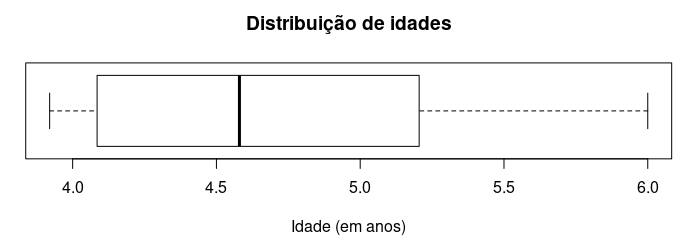
\includegraphics[width=.6\linewidth,fbox]{figs/ages.png}
    \caption{Distribuição de idades.}
    \sourceauthor
    \label{fig:ages}
\end{figure}

Cada sala possui uma professora e uma assistente, denominadas aqui de professoras. Todas são mulheres, e possuem de 4 a 28 anos de experiência de trabalho com crianças. Das seis professoras participantes, três responderam diretamente a entrevistas e outras três colaboraram em algum momento por meio de comentários a respeito do projeto ou auxiliando na comunicação com as crianças. As nomes utilizados no texto são fictícios, a fim de evitar a identificação dos participantes
\footnote{
    O guia \textit{Orientações para relato de Pesquisa Qualitativa envolvendo Tecnologias Educacionais}, do \ac{CIEB}, sugere também descrever o pesquisador como um participante. O pesquisador é um sujeito que nunca está ausente, e suas vivências e experiências anteriores impactam a compreensão do fenômeno em estudo. O pesquisador do presente trabalho é um homem de 26 anos, com formação em computação e experiência em desenvolvimento de softwares para empresas. Em estudos anteriores na universidade desenvolveu interfaces para o brinquedo RoPE. Nessa experiência as crianças interagiram via aplicativo, e o pesquisador dificuldade das crianças usarem o smartphone, pois que não conseguiam arrastar elementos na tela. No mesmo trabalho considerou o smartphone como um dispositivo inadequado para o ambiente de um CDI, pois havia o medo de que alguma criança o quebrasse. A interação das crianças apenas com elementos tangíveis seria uma alternativa a esses problemas, pois manipular objetos tangíveis é atividade rotineira nos CDIs. Essas experiências prévias podem representar viéses desta pesquisa e uma ameaça à validade dos resultados.
}.

O recrutamento, portanto, se deu por conveniência. As crianças participantes frequentavam o ambiente no dia da visita do pesquisador. Não houve distinção de sexo ou presença/ausência de deficiência intelectual. A ordem de participação das crianças se deu com o pesquisador solicitando à participação de crianças e as professoras selecionando as crianças. As crianças que quiseram participar antes da solicitação não foram impedidas. Deste modo não houve um controle rígido do acesso à interface, mas sim uma organização para evitar mais de três crianças utilizando ao mesmo tempo. Quanto às professoras, participaram das entrevistas as responsáveis pela turma em questão ou as que se sentiram confortáveis em responder.

\section{Ambiente}
As atividades ocorreram em três salas comumente frequentadas pelas crianças. Em todas as salas o projetor ficou em um suporte, posicionado ao lado de uma fonte de energia e afastado de janelas e portas. As luzes das salas foram apagadas, mas isso não modificou o ambiente a ponto de torná-lo escuro (ver \autoref{fig:setting}). No chão, à frente do projetor, foram fixadas duas cartolinas brancas para receber as imagens projetadas. Ao lado do projetor um notebook foi posicionado para servir como câmera. 

\begin{figure}[!h]
    \centering
    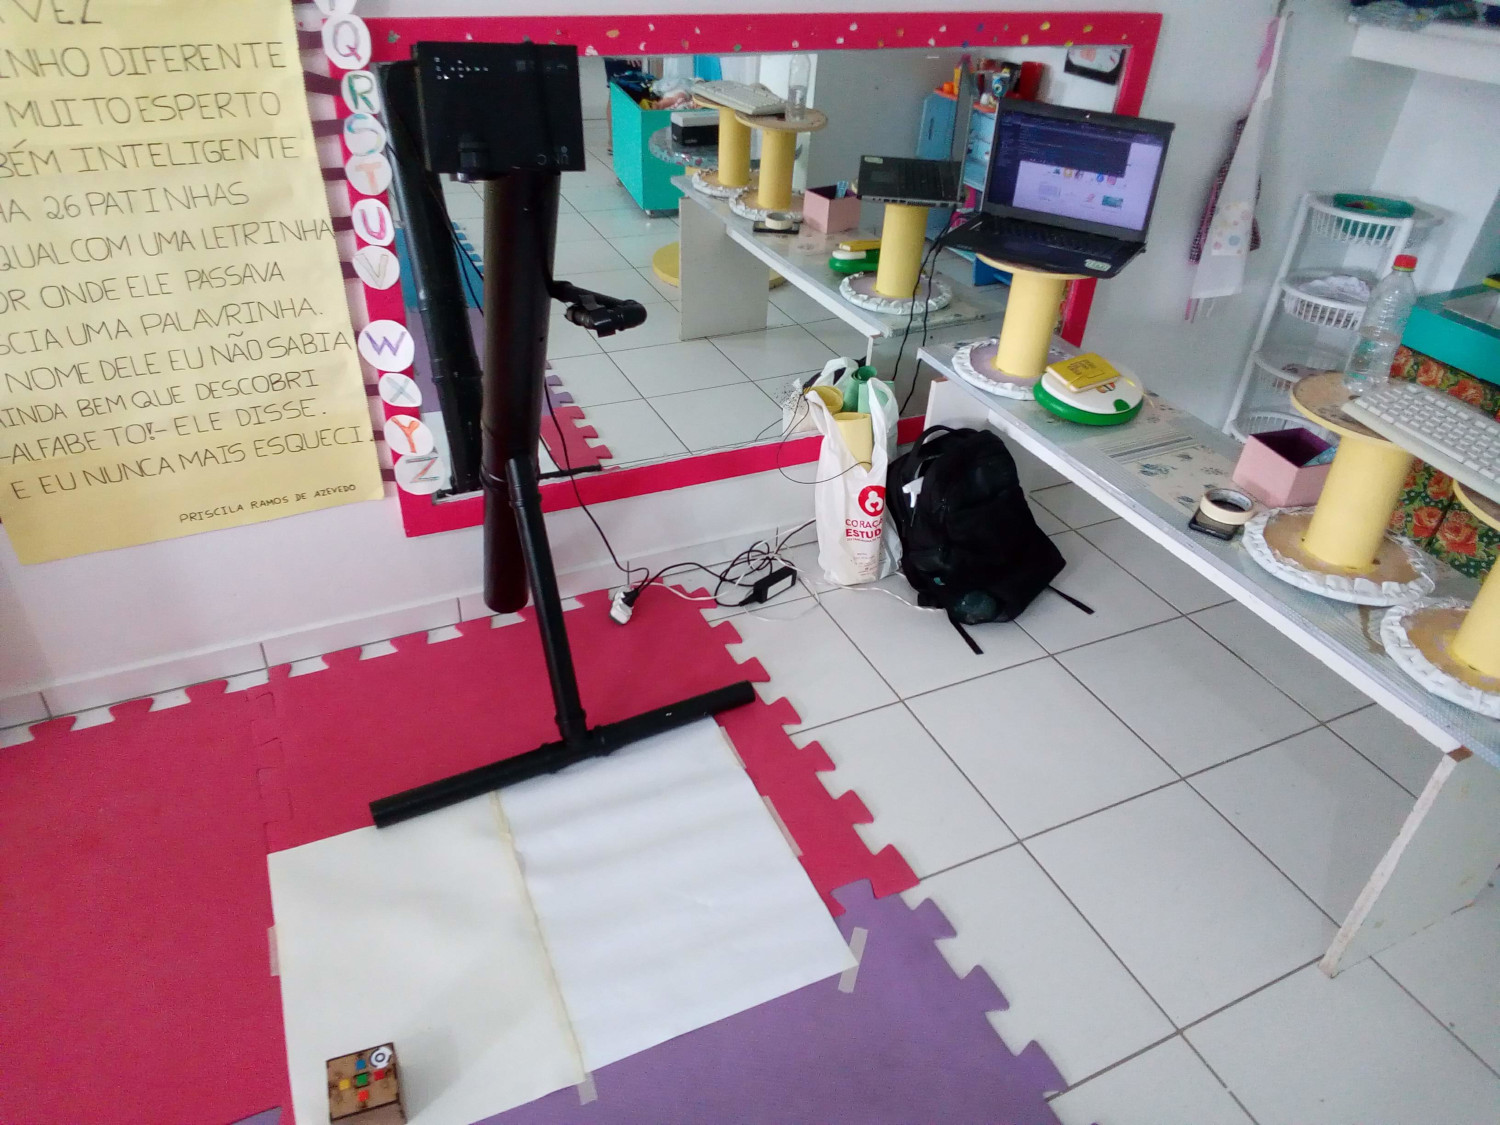
\includegraphics[width=0.8\textwidth,fbox]{figs/setting_projector.jpg}
    \caption{Posicionamento do projetor.}
    \label{fig:setting}
\end{figure}

As crianças continuaram suas atividades junto às professoras enquanto o pesquisador organizava os equipamentos. Era perceptível a curiosidade das crianças a respeito dos materiais e da figura do pesquisador, tanto pelos olhares quanto por perguntas feitas às professoras. Ao lado da sala da turma 4-5A há um espaço externo gramado. Neste ambiente a professora continuou as atividades no espaço externo, e a programação do RoPE ocorreu dentro da sala com a outra professora presente. As outras duas salas tem espaços amplos, e todas as crianças permaneceram no recinto durante a atividade. Enquanto duas ou três participavam da pesquisa, as demais continuavam suas atividades em uma outro ponto da sala.

O CDI tem rede de internet sem fio, porém a qualidade do sinal é variável em cada sala. Especificamente na sala 4-5A há dificuldade de manter a conexão. Esse problema foi mencionado pelas professoras e ocorreu durante a conexão do projetor na rede. As demais salas visitadas, porém, tem conexão estável.

\section{Materiais e Protocolo de Coleta de Dados}
\label{sec:protocolo}
Após a organização do ambiente ocorreu o contato das crianças com a RoPE AR. Esse contato seguiu um roteiro com cinco etapas: seleção dos participantes, ambientação, reconhecimento dos blocos, programação e depuração. O roteiro serviu como base mas não impediu flexibilizar as atividades, de modo a se adaptarem às sugestões das crianças, dificuldades, curiosidades, e restrições de tempo existentes.

O trecho a seguir descreve o protocolo seguido. Os rótulos [MAT] e [ETAPA] destacam os materiais utilizados e as etapas.

\relato{
    Após ajustar o projetor [MAT PROJETOR] no suporte [MAT SUPORTE] e iniciar a gravação com a câmera do notebook [MAT CÂMERA], o pesquisador perguntou quais crianças gostariam de iniciar a brincadeira. A professora perguntou quantas crianças poderiam participar por vez, e o pesquisador respondeu que o ideal seria um grupo de duas ou três crianças [ETAPA 1 - SELEÇÃO]. A professora então chamou duas crianças pelo nome, que interromperam suas atividades junto às demais e se dirigiram até o pesquisador.

    As duas crianças e o pesquisador se sentaram em um tapete, visível na câmera. Para ambientar as crianças e fazê-las se sentirem mais confortáveis [ETAPA 2 - AMBIENTAÇÃO], o pesquisador se apresentou e pediu para as crianças falarem seus nomes e idades, e em seguida apresentou a atividade: "Hoje nós vamos conhecer um robô. Vocês conhecem algum robô? Como ele é? O que ele faz?". Cada criança respondeu se conhecia ou não algum robô, geralmente mencionando brinquedos ou personagens de desenhos animados. Depois da conversa inicial, o pesquisador apresentou o RoPE [MAT ROPE] e os blocos de papelão [MAT BLOCOS]. Para cada bloco, perguntou [ETAPA 3 - COMPREENSÃO DOS SÍMBOLOS DOS BLOCOS]: "O que vocês estão vendo neste desenho aqui?". Em caso de resposta errada ou ausência de resposta, o pesquisador perguntou: "O que o robô está fazendo?". Também buscou observar como as crianças encaixavam os blocos, quais relacionamentos percebiam entre os blocos e os botões do brinquedo. A cada execução do robô, o smartphone enviou os comandos informados para a CtPuzzle Platform [MAT CONEXÃO COM A INTERNET].

    Após o reconhecimento dos blocos, o aplicativo [MAT SMARTPHONE] e a projeção foram ligados. O pesquisador perguntou o que as crianças viam na área projetada, e essas responderam que estavam vendo uma maçã. O pesquisador explicou às crianças que deveriam ajudar o RoPE pegar a maçã, andando pelo caminho marrom, e para isso deveriam usar os blocos [ETAPA 4 - PROGRAMAÇÃO]. Para a primeira maçã o pesquisador explicou o funcionamento: colocou o RoPE na posição inicial, encaixou o bloco Frente (azul) no bloco Início (verde) e apertou o botão verde (iniciar) do RoPE. O brinquedo andou para frente e capturou a maçã. As crianças então usaram os blocos e programaram o robô para pegar as próximas quatro maçãs. Dúvidas e erros surgiram com frequência, e o pesquisador auxiliou fazendo perguntas e dando exemplos quando necessário, e explicando as regras e direções.
    
    Após a captura das 5 maçãs na primeira etapa, iniciou a etapa de depuração [ETAPA 5 - DEPURAÇÃO]. O pesquisador sequenciou os blocos de forma a haver um erro que faria o RoPE não pegar a maçã, e solicitou às crianças que tentassem encontrá-lo. Nos casos em que as crianças não encontraram o erro imediatamente, o pesquisador pediu para apertarem o botão verde e ver o robô andar na direção errada, para então corrigirem o erro. Vendo o movimento errado do robô, as crianças então modificaram o algoritmo para eliminar o bug. Quatro bugs foram encontrados, e então a brincadeira terminou. O pesquisador agradeceu às crianças, e perguntou se o vídeo da atividade poderia ser usada no seu trabalho. Para isso apresentou dois rostos em uma folha pequena, um alegre e um triste. As crianças consentiram no uso do vídeo pintando o rosto alegre [MAT FOLHA DE CONSENTIMENTO].
}

Como descrito, a etapa 4 (programação) tem 5 fases (\autoref{quadro:fases_programacao}). A complexidade da solução de cada uma dessas fases é crescente. A primeira fase, exige apenas um comando, enquanto a segunda exige dois. A terceira fase também exige dois comandos, porém acrescenta o comando de giro. Além do maior número de comandos, a orientação da criança em relação é outro fator que dificulta a resolução. Nas fases 1 e 2 a criança programa o robô estando na mesma orientação que ele. Nas fases 3 a 5, porém, o robô está com seu lado direito voltado para a criança, e portanto ela precisa imaginar-se em outra perspectiva\footnote{ Piaget e Inhelder (1981) citam a dificuldade que crianças tem de imaginar-se em outra perspectiva (egocentrismo). }.

\begin{quadro}[htbp]
    \captionquadro{Fases de programação}
    \label{quadro:fases_programacao}
    \begin{longtable}{ | m{.2\textwidth} | m{.5\textwidth} | m{.2\textwidth} | }
        \hline
        \textbf{Fase}  & \textbf{Descrição} & \textbf{Solução esperada} \\ \hline
        \endhead
        
        %%%%%%%%%%%%%%%%%%%
    
        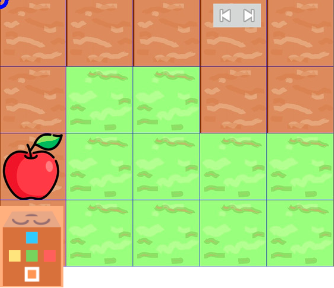
\includegraphics[width=.9\linewidth]{figs/prog/1.png} &
    
        \textbf{Fase 1}: 
        Primeira fase e a mais simples. O desafio é andar apenas um passo à frente. A intenção é que a criança compreenda que o robo se move em correspondência ao bloco encaixado, e que o início da execução ocorre ao apertar o botão verde do robô. &
        
        Frente

        \\ \hline
    
        %%%%%%%%%%%%%%%%%%%
    
        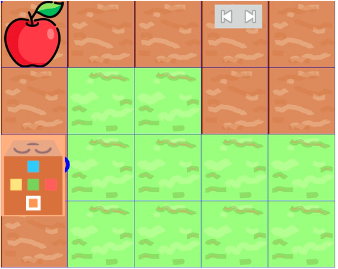
\includegraphics[width=.9\linewidth]{figs/prog/2.png} &
    
        \textbf{Fase 2}: 
        A ideia aqui é que a criança compreenda que o robô faz mais de um passo por vez. Precisa justapor dois blocos frente para alcançar o objetivo. & 
        
        Frente, frente

        \\ \hline
    
        %%%%%%%%%%%%%%%%%%%
    
        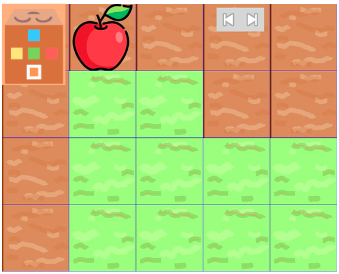
\includegraphics[width=.9\linewidth]{figs/prog/3.png} &
    
        \textbf{Fase 3}: 
        Nesta fase é adicionada o movimento de giro. A maçã aparece do lado direito do robô, que está virado para frente. &

        Direita, frente
        
        \\ \hline
    
        %%%%%%%%%%%%%%%%%%%
    
        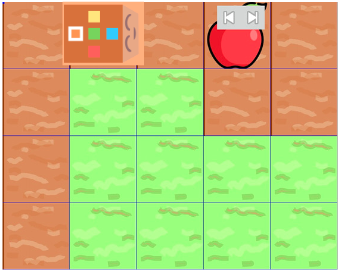
\includegraphics[width=.9\linewidth]{figs/prog/4.png} &
    
        \textbf{Fase 4}:
        A solução desta fase emprega os mesmos comandos que a Fase 2. A diferença é a orientação provável do robô em relação à criança. Se a criança estiver na frente da área projetada, então verá a lateral direita do RoPE. Na Fase 2 criança e robô estão em orientações iguais. &

        Frente, frente
        
        \\ \hline
    
        %%%%%%%%%%%%%%%%%%%
    
        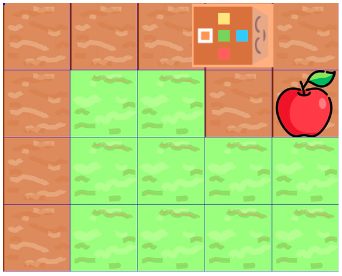
\includegraphics[width=.9\linewidth]{figs/prog/5.png} &
    
        \textbf{Fase 5}: 
        Esta é a fase de programação que exige maior número de comandos (três). Além disso a criança precisa imaginar a posição do robô após o giro, para então decidir o comando a ser usado em seguida (frente).
        &
        Frente, esquerda, frente 
        
        \\ \hline
        
    \end{longtable}
\end{quadro}

A depuração é a quinta etapa do protocolo (\autoref{quadro:fases_depuracao}). Enquanto na programação a criança \textit{escreve} código justapondo os blocos, a depuração favorece a \textit{leitura} de código. Há quatro fases, em ordem crescente de dificuldade. Em cada uma há um bug, que faz o brinquedo ir em uma direção errada e não capturar a maçã. Na Fase 6, por exemplo, o bug é um comando de avanço à esquerda, quando o correto seria um avanço à frente. A atividade consiste, então, na criança olhar, discutir, modificar e testar o algoritmo para eliminar o bug e resolver o problema.

\begin{quadro}[htbp]
    \captionquadro{Fases de depuração}
    \label{quadro:fases_depuracao}
    \begin{longtable}{ | m{.2\textwidth} | m{.5\textwidth} | m{.1\textwidth} | m{.1\textwidth} |}
        \hline
        \textbf{Fase}  & \textbf{Descrição} & \textbf{Solução esperada} & \textbf{Tipo de erro} \\ \hline
        \endhead
        
        %%%%%%%%%%%%%%%%%%%
    
         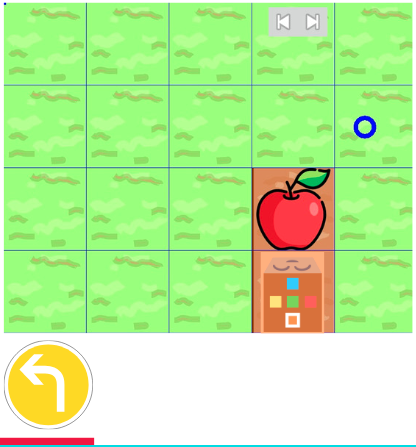
\includegraphics[width=.9\linewidth]{figs/debug/1.png} &
    
         \textbf{Fase 6}: 
         A maçã está logo à frente, porém o algoritmo tem um giro à esquerda. & 
         
         Frente & Comando incorreto
 
         \\ \hline
     
         %%%%%%%%%%%%%%%%%%%
     
         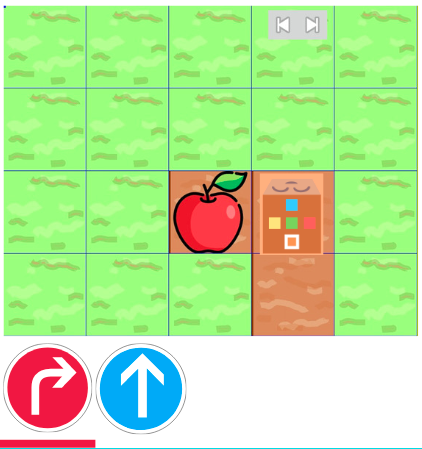
\includegraphics[width=.9\linewidth]{figs/debug/2.png} &
     
         \textbf{Fase 7}: 
         Nesta fase o erro é o comando de giro. O robô precisa girar à esquerda, mas o comando utilizado é o de girar à direita. &
 
         Esquerda, frente & Comando incorreto
         
         \\ \hline
     
         %%%%%%%%%%%%%%%%%%%
     
         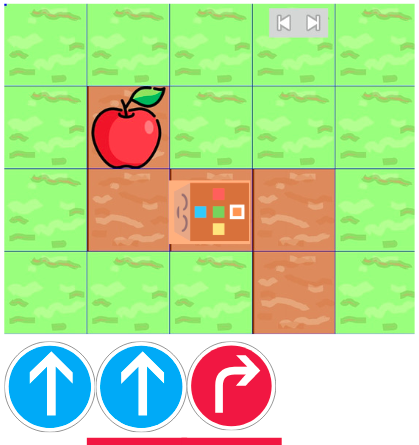
\includegraphics[width=.9\linewidth]{figs/debug/3.png} &
     
         \textbf{Fase 8}:
         O erro nesta fase está na ordem dos comandos utilizados. Se o brinquedo avança duas vezes ele passa da posição onde deve girar à direita. A tarefa consiste em reordenar os comandos já existentes, em vez de adicionar ou remover comandos. &
 
         Frente, direita, frente & Ordem dos comandos
         
         \\ \hline
     
         %%%%%%%%%%%%%%%%%%%
     
         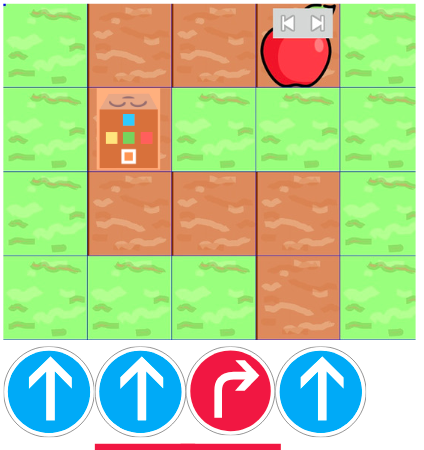
\includegraphics[width=.9\linewidth]{figs/debug/4.png} &
     
         \textbf{Fase 9}: 
         Tarefa de maior dificuldade em todas as etapas, pois exige quatro comandos. Assim como na fase 8, o erro está na ordem dos comandos utilizados.
         &
         Frente, direita, frente, frente & Ordem dos comandos
         
         \\ \hline
     
         %%%%%%%%%%%%%%%%%%%

    \end{longtable}
\end{quadro}

Tanto na etapa de programação quanto de depuração, não foi exigida a finalização de todas as fases. Pesquisador e professora decidiram interromper as atividades em casos onde as crianças apresentaram sinais de cansaço ou perderam atenção à tarefa. Além disso, as 9 fases definidas serviram como uma base, mas não como uma restrição. Ocorreram modificações de trajeto, onde a criança sugeriu um outro ponto de partida ou um caminho mais longo. Da mesma forma, não foi impedida a resolução do problema em etapas, quando a criança programou o brinquedo para andar até metade do caminho, por exemplo, e depois programou os demais passos.

\subsection{Entrevistas com as professoras}
As entrevistas com as professoras ocorreu individualmente, após as atividades com as crianças. O local da entrevista foi o ambiente escolar, enquanto as crianças prosseguiam com outras atividades, acompanhadas por outra professora. A entrevista ocorreu de forma semi-estruturada, com seis perguntas guia:

\newcommand{\pergunta}[1]{
    \textit{#1}
}

\begin{quadro}[!h]
    \captionquadro{Questionário com as professoras}
    {{\renewcommand{\arraystretch}{1.5}
    \begin{longtable}{| m{.5\linewidth} | m{.5\linewidth}| }
        \hline
        Pergunta & Motivação \\ \hline
        \pergunta{Quais suas experiências e como é o dia a dia do seu trabalho voltado à Educação Infantil?} & Compreender as experiências passadas e o contexto de trabalho da professora. \\ \hline

        \pergunta{O que você pensa sobre crianças tendo contato com tecnologias digitais?} & Identificar possíveis receios em relação à tecnologia e também identificar os dispositivos citados. \\ \hline        

        \pergunta{Que importância você daria para a \destaque{visibilidade} no aprendizado das crianças?} & Verificar se a opinião das professoras se alinha ao diferencial da ferramenta proposta. \\ \hline

        \pergunta{Você poderia pensar em alguma atividade usando os mesmos princípios propostos na atividade de hoje, seguindo a ideia de projetar imagens no chão e ter essa interação com um robô?} & Compreender a percepção do professor sobre a aplicabilidade da proposta. \\ \hline

        \pergunta{Que tipos de problemas você percebe na proposta? Quais aspectos poderiam melhorar? } & \\ \hline

    \end{longtable}
    }
\end{quadro}

\begin{comment}
\begin{itemize}
\item 
\item O que você vê neste desenho? O que está desenhado aqui?
\item Porque você acha que o RoPE está se movendo deste jeito?
\item Como você encaixaria esses desenhos?
\end{itemize}

%A força motriz do design iterativo são as metas do usuário, que são ações que o usuário deseja poder fazer \cite{rogers_design_2013}. Neste trabalho, o alcance das metas de usabilidade se dá quando a criança:

\begin{itemize}
    \item posiciona o brinquedo na posição inicial;
    \item percebe que os blocos representam ações do robô;
    \item sequencia blocos formando um algoritmo;
    \item inicia execução do algoritmo;
    \item altera sequência de blocos; e
    \item percebe blocos destacados durante execução.
\end{itemize}

Para direcionar a observação, as categorias de análise serão 
(i) para quais elementos da interface as crianças olham;
(ii) se e como as crianças manipulam os blocos; 
(iii) perguntas realizadas; 
(iv) se e como as crianças comparam os blocos com os símbolos do robô; 
(v) como ocorre o início da execução; 
(vi) em que local e direção posicionam o robô; e 
(vii) se e como os elementos virtuais são percebidos pelas crianças.

%A colaboração será observada quando duas ou mais crianças brincarem em conjunto com os blocos. Esse tipo de evento já foi observado em estudos anteriores \cite{sapounidis_tangible_2019, raabe_estudo_2019}, mas precisa ser confirmado neste estudo para afirmar que a interface apresentada tem os benefícios das interfaces tangíveis. 

% \cite{bardin_alise_1979}.
\end{comment}